%%%%%%%%%%%%%%%%%%%%%%%%%%%%%%%%%%%%%%%%%%%%%%%%%%%%%%%%%%%%%%%%%%%%%%%%%%%%%%
%
% PROJECT PROPOSAL  DESCRIPTION:
%   A concise description of the main concepts of the proposed project.
%
% RESEARCH:
%   A list of research activities which led to this project.
%
% EXPERIMENTS:
%   A list of the experiments performed which supported the research.
%
%%%%%%%%%%%%%%%%%%%%%%%%%%%%%%%%%%%%%%%%%%%%%%%%%%%%%%%%%%%%%%%%%%%%%%%%%%%%%%%
% Define a single space environment (copied from doublespace.sty)
% e.g. \begin{singlespace}
%         single-spaced text
%      \end{singlespace}

\documentclass[12pt,american]{article}
\usepackage{fullpage}
\usepackage{bbm}
\usepackage{url}
\usepackage{subfigure}
\usepackage{babel}
\usepackage{times}
\usepackage{graphicx}
\usepackage{amssymb}
\usepackage{lscape}
\usepackage{verbatim}
\usepackage{enumerate}
\usepackage{afterpage}
\usepackage{setspace}
\usepackage{listings}
\usepackage{color}
%\usepackage{parskip}

\lstset{numbers=left,
 frame=single,
 captionpos=b,}

\begin{document}
\thispagestyle{empty} 
\begin{center}
{\em MS Project Proposal}\\
\vspace{.5in}
{\large \bf Buffalo: An Aspect Oriented Programming Framework for C\#}\\
\vspace{.5in}
{\bf Wei Liao}\\
\vfill
\
{\em Committee Chair:} Prof. James E. Heliotis\\
\vspace{0.1in}
%Signature: \line(1,0) {100} Date: \line(250, 0) {100}\\
{\em Reader: } Prof. Fereydoun Kazemian\\
 \vspace{0.1in}
{\em Observer: } Prof. Matthew Fluet\\
 \vspace{0.1in}
Department of Computer Science\\
B. Thomas Golisano College of Computing and Information Sciences \\
Rochester Institute of Technology \\
Rochester, New York \\ [0.3in]
\vspace{0.5in}
\today{}\\
\end{center}
\vfill

%%%%%%%%%%%%%%%%%%%%%%%%%%%%%%%%%%%%%%%%%%%%%%%%%%%%%%%%%%%%%%%%%%%%%%%%%%%%%%%
%%  Collection of useful abbreviations.
\newcommand{\etc} {\emph{etc.\/}}
\newcommand{\etal}{\emph{et~al.\/}}
\newcommand{\eg}  {\emph{e.g.\/}}
\newcommand{\ie}  {\emph{i.e.\/}}
%%%%%%%%%%%%%%%%%%%%%%%%%%%%%%%%%%%%%%%%%%%%%%%%%%%%%%%%%%%%%%%%%%%%%%%%%%%%%%%


%%%%%%%%%%%%%%%%%%%%%%%%%%%%%%%%%%%%%%%%%%%%%%%%%%%%%%%%%%%%%%%%%%%%%%%%%%%%%%%
% Abstract
\section*{Abstract}
Aspect Oriented Programming (AOP) is a paradigm that let programmers isolate and separate cross-cutting concerns from the basis of their program. The concept has not been widely adapted by modern languages, support in toolings such as Integrated Development Environment (IDE) is also rare. In this project we will design and implement a framework called Buffalo that provides AOP functionality for C\# via IL code weaving, and integrate it with the Visual Studio IDE build system.
%%%%%%%%%%%%%%%%%%%%%%%%%%%%%%%%%%%%%%%%%%%%%%%%%%%%%%%%%%%%%%%%%%%%%%%%%%%%%%%
\vfill{}

%%%%%%%%%%%%%%%%%%%%%%%%%%%%%%%%%%%%%%%%%%%%%%%%%%%%%%%%%%%%%%%%%%%%%%%%%%%%%%%
% This is where the main body of the capstone proposal starts
\setcounter{page}{0} 
\newpage{}
%\setlength{\parindent}{1cm}
\section{Introduction}
High level object oriented programming languages have given programmers a lot of freedom in expressing themselves in Object Oriented Design. However they are still lacking in some areas when it comes to particular software design decision such as cross-cutting concern~\cite{aop}. 

In this project we will try to solve this type of problem by designing and implementing a framework called Buffalo for the C\# platform, we will show how by using Buffalo programmers can separate those concerns from the core of the program, and ultimately be more productive.

In section 2 we will explain the background of the problem, we will look at some of the areas that the current programming paradigm are not efficient at solving, and illustrate it by look at some examples. In section 3 we will explore the existing works and what have been done. In section 5 we explain what we propose to do and give an overview of the architecture of Buffalo, what we want the end result to be, and how to evaulate it. A tentative roadmap is given in section 6.

\section{Background}
In this section we will explain more about the cross-cutting problem and how AOP can be used to help.

\subsection{The Problem}
Procedural Language such as C achieves modularity by grouping codes into subroutines or functions, whereas Object Oriented Programming (OOP) languages such as JAVA or C\# go one step further, and they allow programmers to abstract real world object into properties and behaviors. Both paradigms give programmers the ability to make their code cleaner and more reusable.

While OOP languages offer data abstraction and encapsulation in the form of objects and classes, the usage of declared instances of all those objects could still be scattered throughout different modules of the program. Overtime, these tangled cross-cutting concerns [1] can be difficult and expensive maintenance. One of the often cited example of such concern is exception handling: the ability to for programs to handle errors or die gracefully.

To handle exception in our code, in its most basic form we can have the follow try..catch block:

\begin{lstlisting}[caption={try..catch pattern}, label=trycatch]
public double Divide(double num1, double num2) {
   try {
       return num1 / num2;
   } catch (Exception e) {
       //log exception to file, etc
       Utility.LogToFile(e);
   }
}
\end{lstlisting}

The code snippet in Listing~\ref{trycatch} illustrated a few key points. First, if {\em num2} is 0, this will cause an exception, and when that happens, execution control is transferred to line 6, where the exception is logged to a file. 

Imagine if you have 1,000 functions in your program that can potentially throw errors, you would have to apply the try..catch block on all of them. And note that the functionality of actually logging the exception is nicely encapsulated in the Utility object, but it does not change the fact that the code is still repetitive, because {\em Utility.LogToFile(e)} still have to be called in 1,000 different places in the source code. Since your program most likely will be consist of different modules, this repetitive pattern will cut through and appears in all the modules.

What if you need to fine tune this try..catch block to catch a specific exception such as the {\em DivideByZeroException} so your program can act accordingly, or instead of using the {\em Utility.LogToFile(e)} you want to use a different object to handle the actual logging. In the worst case you would have to make the change to all 1,000 of your functions.

The problem is how to prevent those cross-cutting concerns from loitering your program. Aspect Oriented Programming technique [1] can be used to cleanly separate such concerns.

\subsection{Aspect-Oriented Programming}
The Aspect Oriented Programming paradigm was first discussed in the 1997 paper~\cite{aop}. When talking about AOP, the following concepts are worth noting.

{\em concern} - It is the repetitive code that cross-cut into different modules of the program. It is often code that does not conviently fit into the dominant paradigm of design.

{\em aspect} - It is the piece of isolated code that can be used to solve the issue of a particluar concern.

{\em join points} - These are the locations through out the program where the concern is leaked into, it is also where the aspect will be applied to solve the concern.

The idea of AOP is fairly simple, we have some code that that appeared and duplicated all over the place, making it difficult to maintaint, so we can isolate that duplicate code into a separate single unit of code, then we can injects that  unit of code into all relevant places in a program either at runtime or compile time, so programmers don't have to do it.

In another word, AOP is about injecting code into a program. This is especially handy when programmers don't have access to the original source code.

\section{Related Work}Most modern programming languages display some AOP-like properties, but full support is rare. Delphi Prism 2010 is one of them, where the weaving of aspect code happens at compile time~\cite{delphi_prism2010}. AOP can be implemented in a variety of ways, but like other programming paradigms, it is most effective and beneficial to programmers when it is supported on the compiler level, making it a first class citizen like other properties of a language.

\subsection{Compile Support}

Gregor Kiczales from the 1997 paper~\cite{aop} started and led the Xerox PARC team developed an implementation of AOP for the JAVA platform called AspectJ. AspectJ is an extension to the JAVA compiler, it is a language in and of itself, with its own specific syntax and usages and even compiler. It produces JAVA VM compatible binary. It would have been nice if this is added directly in the JAVA compiler, which some hopes it will happen soon~\cite{aspectj_faq}. But still, AspectJ integrated nicely with JAVA, especially when used with its own plugin in the Eclipse IDE.

AspectJ can introduce new features to a program, as well as modify it. It provides the {\em aspect} keyword to denote a piece of code as the advice code, the usage is similar to how the {\em class} keyword is used in JAVA.

\begin{lstlisting}[caption={sample aspectj code}, label=aspecjcode]
public aspect MyAspectJ {
   public int Sorter.Count() {
      //do something here
   }
   pointcut doSomething() : call (* * (..));
   before() : doSomething() {
      //do something before calling the actual function
   }
}
\end{lstlisting}

The example in Listing~\ref{aspectjcode} showed how an AspectJ aspect can be defined, suppose we have a class named {\em Sorter}, and we want to add a new method to it but we don't have access to the source code, in AspectJ we can introduce a brand new method to it, as line 2-4 shows. The pointcut {\em doSomething()} does a regular expression match to find all matching functions regardless of access priviledge, names or parameters, which means pretty much every functions in the program. Then line 6-8 means before executing those functions matched, execute the block of code in line 7 first. This effectively created a hook into every single function in a program.

Behind the scene AspectJ piece everything together by bytecode weaving, after JAVA compiles the source, it takes the classes and aspects in bytecode form and weaves them together, producing new .class files that can be loaded onto the virtual machine.

Despite Eclipse's claim that AspectJ is very easy to learn, one of the disadvantage of AspectJ is, as the above example shows, the syntax is somewhat different from a normal JAVA program, making the learning curve much deeper, but we agree that once get used to it AspectJ can be a really powerful tool for a programmer~\cite{aspectj_text}.

\subsection{Framework Support}

AspectJ is one of the few compiler that does AOP, for the vast programming languages out there, support is provided via some sort of frameworks. This is especially true on the C\# platform~\cite{aopcs}, where Microsoft has indicated that they will not be integrating support for AOP on the C\# compiler anytime soon. Although their Patterns \& Practice team release Policy Injection application block that offer some AOP capability.

There are a number of frameworks available for the C\# platform, they come in various flavors and implemented with different technique. There are several approaches and each has its advantages and disadvantage.

One of the most common implementation involves the usage of a proxy, where the client does not interact with the objects directly, everything goes through the proxy.

\begin{figure}[here]
  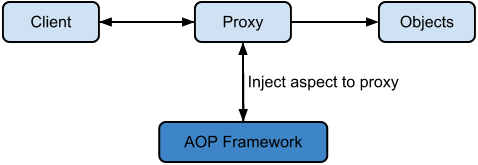
\includegraphics[scale=0.70]{proxy.png}
  \caption{AOP framework using proxy\label{proxy_model}}
\end{figure}

By using the proxy this provides an opportunity for the injection of code to it. The advantage of this approach is relatively ease of implementation, but it is also limiting in that in order for the proxy to work, both the proxy and the target object must implement the same interface, therefore the aspect injection point can only occur in the defined functions in the interface. Since this require reflection at runtime to generate the proxy, the performance is usually not as good.

Another approach is similar to AspectJ, where bytecode weaving is involved, but without the extra complexity of a new syntax and language. The commercial product PostSharp~\cite{postsharp} is an example, where aspect weaving happens post compilation by rewriting MSIL instruction set, PostSharp use just the standard C\# language, attribute is used as advice code, the advantage is ease of use, developer already familiar with C\# will have no learning curve at all. And since aspect is woven in the assembly, the runtime has no overhead of reflection and therefore performance is good. Disadvantage being, since it has to work with MSIL instruction set, it is very low level and therefore the most difficult to implement.

Some frameworks use static weaving~\cite{aspectcs}, where the source files are pre-processed to include all the relevant aspect code, then just let the C\# compile take over and does the compilation normally. This has the advantage of post compilation weaving but not the MSIL complexity. On the other hand, you do have to develop a parsar generator to efficiently parse the source files.

\section{Hypothesis}
The OOP paradigm cannot efficiently solve the cross-cutting problem, we believe those problems can be solved efficiently at the compiler level, where it logically belongs.

Even-though the C\# compiler will not support the AOP paradigm, we can still archieve the same goal by doing the separation of concern for them via Buffalo, and further ease the developer's life by hooking Buffalo into the MSBuild system. So developers can focus on just creating the aspects to solve the problems.

\section{Approach and Methodology}
In this section we will give an overview of the architecture of Buffalo, the tools and approach we will be using to implement it.

\subsection{Architecture Overview}
The approach we plan to take is to perform post compilation weaving. Figure 1 shows an overview of how Buffalo will fit in the overall C\# compilation process.

\begin{figure}[here]
  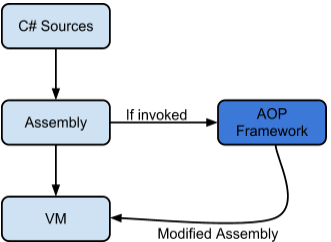
\includegraphics[scale=0.70]{model_overview.png}
  \caption{Buffalo model overview\label{buffalo_model}}
\end{figure}

\subsection{Post Compilation Weaving}
As Figure~\ref{buffalo_model} shows, the C\# compiler compiles the source files into an assembly, this assembly is then fed into Buffalo. Buffalo takes apart the assembly using reflection to find all the defined {\em aspects} and {\em pointcuts}, then rewrite the MSIL instruction set, weaving in the {\em aspects} into the right places, finally producing a new assembly.

Once C\# finishes the compilation, the control is transfer to Buffalo, this step is archieved by creating a hook into the MSBuild system. If Buffalo detects any {\em aspects} defined in the input assembly, and the {\em aspects} are being applied, the weaving will take place, otherwise the whole process will be ignored.

\subsection{Intended Usage}
From the Visual Studio IDE, developer can use Buffalo by first creating a custom C\# attribue, extending a Buffalo interface IAspect (subject to change), for ex:

\begin{lstlisting}[caption={Buffalo aspect}, label=buffalocode]
public class CatchException : System.Attribute, IAspect {
   public void OnException(Exception e) {
       Utility.LogToFile(e);
   } 
}
\end{lstlisting}

Now {\em CatchException} will be treated as an aspect by Buffalo, to use it, simply use it like a regular attribute and apply it to any method, class or assembly.

\begin{lstlisting}[caption={applying Buffalo aspect}, label=applybuffalo]
[CatchException]
public double Divide(double num1, double num2) {
   return num1 / num2;
}
\end{lstlisting}

As the code snippets in Listing~\ref{applybuffalo} shows, the cross-cutting concerns is now cleanly separated into a cutom attribute {\em CatchException}, any change made to the aspect will be propogated to all the annontated functions. As a result. By applying this attribute to the functions, the repetitive try..block is no longer necessary, the target code is much shorter and cleaner. 

The real benefit will be more evident when an aspect is apply to a large number of functions, or asemblies, for ex, if I want every function within every class to be able to catch exception:

\begin{lstlisting}[caption={applying Buffalo aspect on an assembly}, label=applybuffaloassembly]
[CatchException]
namespace MyAssembly {
   public class MyClass {
      public double Divide(double num1, double num2) {
         return num1 / num2;
      }
      //other functions...
   }
   //other classes...
}
\end{lstlisting}

By applying the attribute on the assembly level, a single line of code, this will effectively allow every function to have exception handling capability. This will be a huge developer productivity gain.

\subsection{Platform, Languages and Tools}
This project will be developed using C\#, on the Windows 7 using Visual Studio 2010. When performing IL rewriting there are a few options available, one is to use the Reflection.Emit library that comes with the .NET Framework, however all researches points to that this library represents only a subset of the MSIL instructions, the missing instruction might prove to be a problem later on.

Another option is to use the Profiler API by Microsoft, but this API is intended as a debugging feature, and therefore is unsuitable to be used in production environment.

While we can opt to invest the time on learning and rolling a custom MSIL rewriter, we are afraid that in itself is a bigger project than Buffalo~\cite{msil_text}. So a more practical option is to use a third party library. Mono is an open source implementation of the C\# compiler, Cecil is a project within the Mono that provides MSIL rewriting. Preliminary evaluation of the tool seems to be pretty feature complete and flexible enough to allow me to do what we need to do. However documentation for Cecil is next to non-existent, as it works with low level MSIL, the learning curve is expected to be deep.

The following utility tools will also be heavily used during development: ILSpy, ILDASM and PEVerify. ILSpy is an open source application that dis-assemble assembly to show IL instructions. ILDASM does the same but comes from Microsoft’s .NET Framework. PEVerify is a Microsoft Window SDK tool, it will be used to ensure that the modified assembly produced is a correct assembly, this is something that Cecil does not verify.

\subsection{Measurement}
To evalulate Buffalo, we will show that after using Buffalo, code duplication will be reduced, the cross-cutting concern will be separated into single unit of code where it will be easy to maintain. We will use the {\em Call Hierarchy} feature of Visual Studio to show how many calls issued before and after. 

The code a developer has to write is also considerable less in terms of number of lines, as a result the code will be cleaner and easier to look at, this can also be translated directly into an estimation of development cost saved. We will show the before and after using the {\em Code Analysis} available in Visual Studio.

\section{Roadmap}
The Table~\ref{tab:roadmap_tbl} shows my tentative schedule for the major phases of the project.

\begin{table}[h]
\centering
\begin{tabular}{|l|l|l|}
\hline
Date & Action & Status\\
\hline
07/07/2012 & Pre-Proposal & Accepted\\
07/09/2012 & Proposal & In-progress\\
07/20/2012 & Begin development of Buffalo & In-progress\\
09/10/2012 & Finish development, start testing and analysis & - \\
09/27/2012 & Finish report & - \\
10/10/2012 & Defense & - \\
\hline
\end{tabular}
\caption{Timeline}
\label{tab:roadmap_tbl}
\end{table}

%%%%%%%%%%%%%%%%%%%%%%%%%%%%%%%%%%%%%%%%%%%%%%%%%%%%%%%%%%%%%%%%%%%%%%%%%%%%%%%

%%%%%%%%%%%%%%%%%%%%%%%%%%%%%%%%%%%%%%%%%%%%%%%%%%%%%%%%%%%%%%%%%%%%%%%%%%%%%%%
\bibliographystyle{plain}
% Single space the bibliography to save space.
\singlespacing
\bibliography{Proposal}
%%%%%%%%%%%%%%%%%%%%%%%%%%%%%%%%%%%%%%%%%%%%%%%%%%%%%%%%%%%%%%%%%%%%%%%%%%%%%%%


\end{document}
